\chapter{Implementation of the transformation}
\label{chap:implementation}
%===============================%
%         Trafo stages          %
%===============================%
In this chapter, some details of the transformation implementation will be presented. 

\section{Transformation Stucture}
As mentioned before in section \ref{sec:vsdt}, the transformation process in the VSDT is divided into 5 stages. We've also mentioned that the default validation and structure mapping provided by the transformation framework are reuseable. For the implementation of the new transformation, the framework's DefaultBpmnValidator and BPMN2StrucBPMNTransformation are being reused, as we can see in Figure \ref{fig:implementation_stages}.

\begin{figure}[h]
	\centering		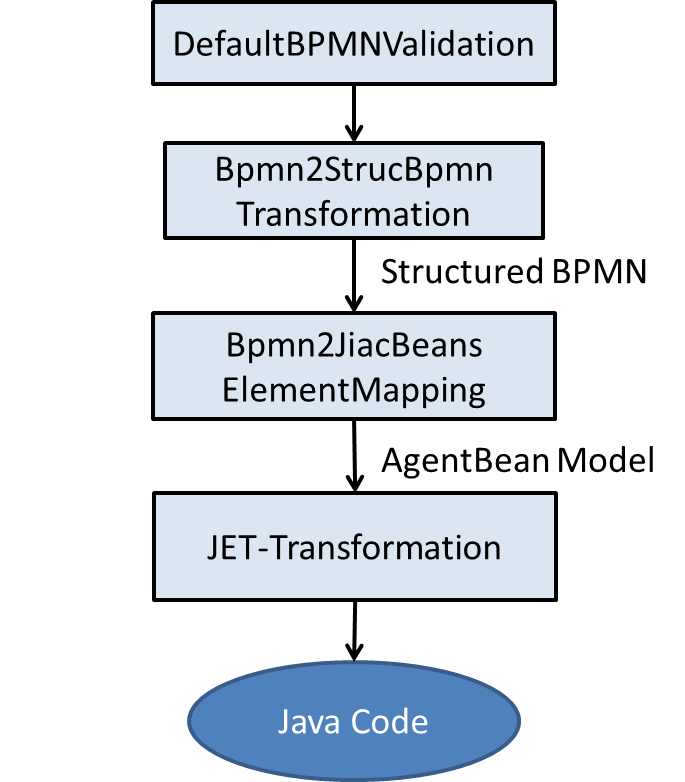
\includegraphics[width=0.5\textwidth]{images/implementation_stages.png}
	\caption{Transformation stages}
	\label{fig:implementation_stages}
\end{figure}

The Element mapping stage is implemented on the basis of the existing Bpmn2JiacV- ElementMapping. It takes a structured Bpmn as a model and transforms each pool contained in the model's business process diagram into a java object, which represent a model of a java file holding an AgentBean class. For this implementation, a Metamodel of the Jiac AgentBean(see Figure \ref{fig:agentbean_metamodel}) was developed as an intermediate product. 

After all Pools in the business process is completely visited and transformed into AgentBean models, these models are passed over to the JET-Transformation where they will be transformed into a String which represents the content of a Java File. 

%===============================%
%       Element Mapping         %
%===============================%
\section{AgentBean Model}

An AgentBean model has a list of attributes, methods, action and it may also have some subprocess(because a subprocess is mapped into an inner class of the generated AgentBean).\\\\
For the content of a Method, a Script-Model was also developed. A script is basically a java code element, which can be a single CodeElement(a single line java code), a sequence which contains a list of scripts, or even a block construct such as the while loop, or a try-catch block. 

\begin{figure}[h]
	\centering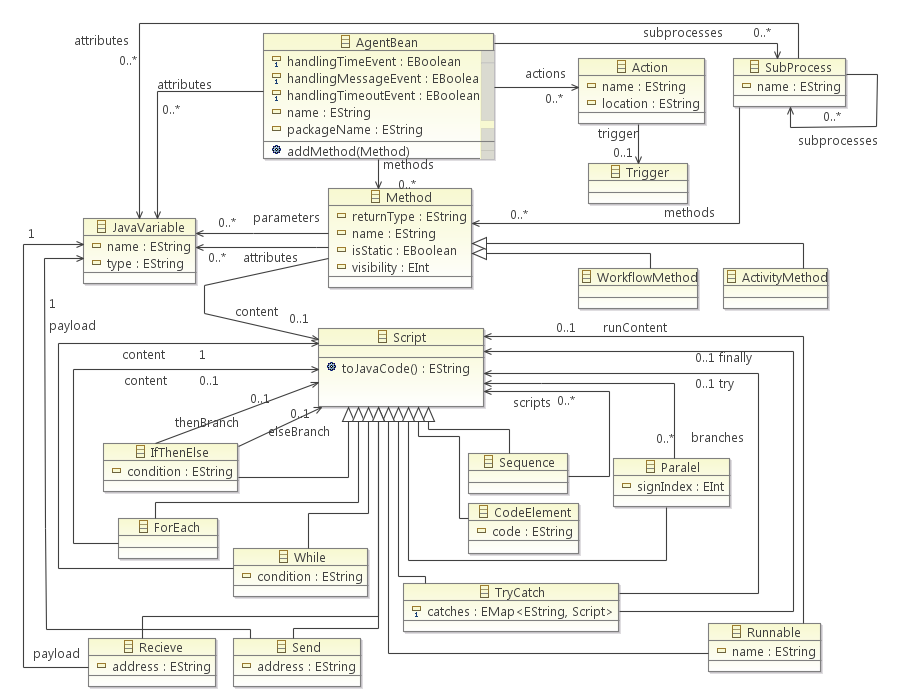
\includegraphics[width=1.0\textwidth]{images/agentBean_metamodel.png}
	\caption{AgentBean - Metamodel}
	\label{fig:agentbean_metamodel}
\end{figure}
\newpage
Each script implements the method \lstinline[language=Java]{public String toJavaCode()} which returns the java code representation of the script.
In the following listing we can see the implementation of the method in the IfThenElse class:
\begin{lstlisting}[language = Java, caption = toJavaCode() implementation in the IfThenElse class]
	public String toJavaCode() {
		String code = "";
		code += "if("+condition+"){\n";
		if(thenBranch!=null){
			BufferedReader reader = new BufferedReader(new StringReader(thenBranch.toJavaCode()));
			try{
				String line = reader.readLine();
				while(line!=null){
					if(!line.equals("")) code += "\t"+line+"\n";
					line = reader.readLine();
				}
			}catch(IOException e){
				code += "\t//Error occured while reading if branch\n";
			}
		}
		code+="}";
		if(elseBranch!=null){
			code+="else{\n";
			BufferedReader reader = new BufferedReader(new StringReader(elseBranch.toJavaCode()));
			try{
				String line = reader.readLine();
				while(line!=null){
					if(!line.equals("")) code += "\t"+line+"\n";
					line = reader.readLine();
				}
			}catch(IOException e){
				code += "\t//Error occured while reading else branch\n";
			}
			code+="}";
		}
		return code;
	}
\end{lstlisting}

You might notice, that this method is also responsible for the text formatting because this method will be used by the JET-Transformation and the result will then be written in a *.java File. Therefore, as you can see in line 7-11 and 21-25, a tab are added in front of each line in the then and else branch.\\\\
%%%%%%%%%%%%%%%%%%%%%%%%%%%
% Role of MDE             %
%%%%%%%%%%%%%%%%%%%%%%%%%%%
\textbf{The role of MDE in the Implementation}\\\\
The benefits of Model Driven Engineering are also found during the implementation of the AgentBean model. As we can see in Figure \ref{fig:agentbean_metamodel}, it is created graphically using eclipse's Ecore Tools - Ecore Diagramm. With the help of the EMF Generator each element of the model can be easily generated into JavaCode including a Factory class that can be used to instantiate an object of each generated class. This way, we only have to implement the method toJavaCode() for each newly added script, everything else are generated automatically. 



%%%%%%%%%%%%%%%%%%%%%%%%%%%%%%%%%%%%%%%%%%%%%%%%%%%%%%%%%%%%%%%%
%								        JET-Transformation                     %
%%%%%%%%%%%%%%%%%%%%%%%%%%%%%%%%%%%%%%%%%%%%%%%%%%%%%%%%%%%%%%%%
\section{JET-Transformation}





%%%%%%%%%%%%%%%%%%%%%%%%%%%%%%%%%%%%%%%%%%%%%%%%%%%%%%%%%%%%%%%%
%           Merging generated and manually edited code         %
%%%%%%%%%%%%%%%%%%%%%%%%%%%%%%%%%%%%%%%%%%%%%%%%%%%%%%%%%%%%%%%%
\section{Merging generated and manually edited code}
One of the challenge in generating java code is how to handle code that has been manually edited.
